\section{Numerical Tests}

\subsection{Cases Configuration}

The setup is shown in Fig. \ref{fg:config}, where the heavy (liquid) and light (gas) phases are represented with gray and white colors respectively. The distance $h$ between the cylinder top and the undisturbed free surface is taken as the measure of the cylinder submergence. Uniform inflow velocity with module $U$ is imposed on the inlet. The chosen Froude number based on the diameter of the cylinder $d$ is defined as
\begin{equation}
 Fr = \frac{U}{\sqrt{gd}}
\label{eq:froude}
\end{equation}
where $g$ is the gravity acceleration. Also, the Reynolds number based on the inlet velocity $U$ and the cylinder diameter $d$, is calculated as
\begin{equation}
 Re = \frac{\rho_l U d}{\mu_l}
\label{eq:reynolds}
\end{equation}
being $\rho_l,\mu_l$ the density and the dynamic viscosity of the heavier phase.


In the reference work of Reichl et.al \cite{Reichl05}, densities and viscosities ratios are established in $\rho_l/\rho_g = \mu_l/\mu_g=100$ in order to avoid convergence problems. PFEM-2 method does not suffer from these drawbacks, allowing more realistic water-air ratios. However, the original ratios are employed to guarantee same simulation conditions. Regarding the boundary conditions, a uniform flow with velocity $U$ is imposed at the inlet boundary, and typical FEM natural boundary condition is used for the top and outflow boundaries. The floor of the channel and the cylinder surface are considered as no-slip walls.

\begin{figure}[htbp]
  \begin{center}
    \subfloat[$Fr=0.3$]{
	  \label{fg:vort_a}
	  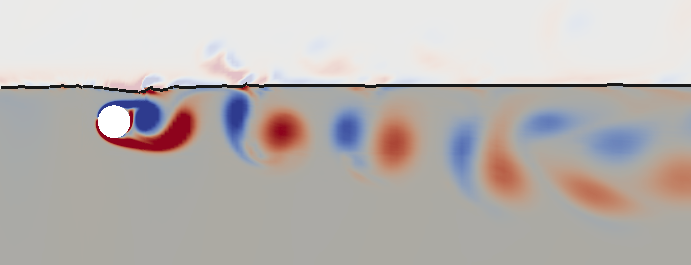
\includegraphics[width=.9\columnwidth]{../images/Fr_0_3_Re_180_h_0_55_vorticity.png}
    } \\
\subfloat[$Fr=0.6$]{
	  \label{fg:vort_b}
	  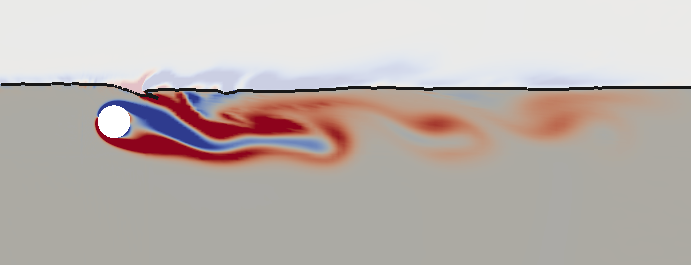
\includegraphics[width=.9\columnwidth]{../images/Fr_0_6_Re_180_h_0_55_vorticity.png}
    } \\
\subfloat[$Fr=0.8$]{
	  \label{fg:vort_c}
	  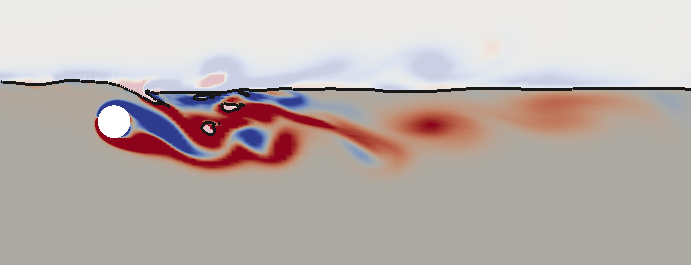
\includegraphics[width=.9\columnwidth]{../images/Fr_0_8_Re_180_h_0_55_vorticity.png}
    } \\
\subfloat[$Fr=1.2$]{
	  \label{fg:vort_d}
	  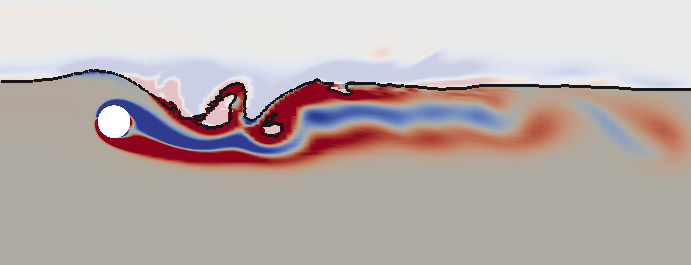
\includegraphics[width=.9\columnwidth]{../images/Fr_1_2_Re_180_h_0_55_vorticity.png}
    } \\
\subfloat[$Fr=1.6$]{
	  \label{fg:vort_e}
	  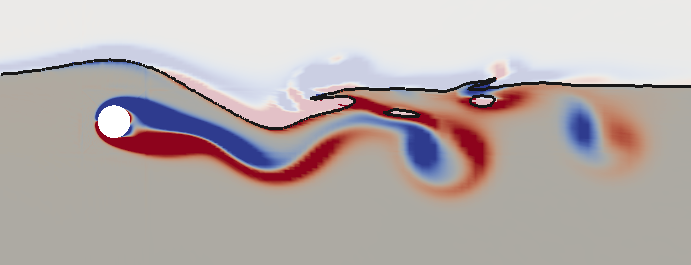
\includegraphics[width=.9\columnwidth]{../images/Fr_1_6_Re_180_h_0_55_vorticity.png}
    } \\
\subfloat[$Fr=2.0$]{
	  \label{fg:vort_f}
	  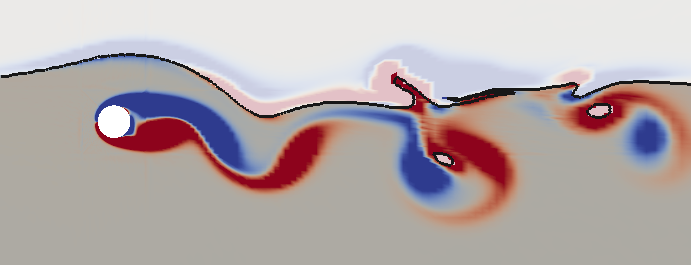
\includegraphics[width=.9\columnwidth]{../images/Fr_2_0_Re_180_h_0_55_vorticity.png}
    } \\
% \subfloat[$Fr=3.5$]{
% 	  \label{fg:vort_g}
% 	  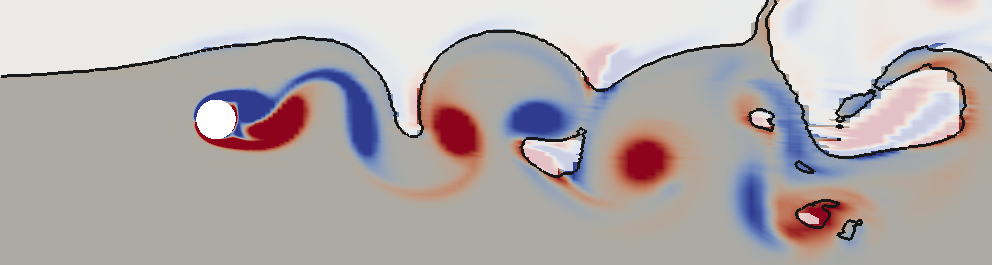
\includegraphics[width=.9\columnwidth]{../images/Fr_3_5_Re_180_h_0_55_vorticity.png}
%     } \\
  \end{center}
  \caption{Influence of Froude number on dimensionless vorticity $\hat\omega = curl(\vv) \sqrt{d/g}$ (scales from -3 (blue) to 3 (red)) with $h/d = 0.55$ and $Re=180$. Captures at $t^*=80$.
}
\label{fg:vort_Re180}
\end{figure}

Flow conditions are inspirated in the work of Bouscasse \cite{Bouscasse14} which investigates the flow behavior employing a range of Froude numbers ($Fr=0.3$, $0.6$, $0.8$, $1.2$, $1.6$ and $2.0$) for a fixed submergence ratio ($h/d=0.55$) and a fixed Reynolds number of $Re=\frac{\rho_l U d}{\mu_l}=180$.

As it was explained in the introduction, one of the advantages of using SPH as numerical method allowing is to treat larger fragmentation of the free surface, when compared to FLUENT-VOF technique used by Reichl and colleagues. The PFEM-2 method employed in the current work, since its particle nature, is also able to treat large deformations and breakups, but, due to the use of the temporal integrator named XIV-S \cite{Idelsohn12}, it can manage larger time steps resulting in shorter computing times \cite{Gimenez2015186}. PFEM-2 simulations were carried out employing the implementation presented in \cite{Gimenez14}. The maximum $CFL=\Delta t U/\Delta x$ allowed in each simulation was $CFL_{max}<8$, in contrast with the small time-steps typically needed by SPH. This feature entails a diminishing in the total computing time to solve the same problem, showing the goodness given by PFEM-2 to solve convective-dominant problems.

\subsection{Simulation Results}

Figure \ref{fg:vort_Re180} shows the influence of the Froude number in the flow characteristics, represented by the dimensionless vorticity. Due to the PFEM-2 is a two-phase solver, in the plots the air regions are presented with some transparency in order to remark the water regions. When the lowest Froude number is imposed $Fr=0.3$, the free-surface deforms very little behaving as a no-slip wall where the vorticity presents a distribution similar to the cases where only one-phase is used \cite{PRICE2002175}. As the Froude number increases $Fr=0.6$, the velocity and vorticity fields change substantially. Although the free-surface just deforms in the proximities of the cylinder, the vortex shedding process has been substantially reduced. Another important observation is that, a recirculation area appears just behind the cylinder and close to the free-surface, the positive vorticity generated at the free surface by the spilling breaker builds up a large positive meta-vortex behind the cylinder which is then advected downstream. Reaching intermediate-high Froude numbers (1.2) structures developed are not periodic, while as the vortex production remains blocked due to the continuous breakups occurring at free-surface. Although the non-stationary behavior of the flow at free-surface, this phenomena allows to obtain constant forces acting over the cylinder. Analysis and discussions presented in this paragraph are in agreement with the work of Bouscasse et. al \cite{Bouscasse14}.

When the analysis for $Fr=1.6$ is done, some differences between the flow characteristics of Bouscasse et. al \cite{Bouscasse14} and the present work are found. Bouscasse shows that at this Froude number the vortex shedding remains blocked while the current results find that it is almost recovered. In order to present a regime where a structure similar to a Von Karman street appears, cases with $Fr=2.0$ and $3.5$ were also run finding vortex shedding behind the cylinder and large distortions of the free-surface but without the characteristic chaos of the intermediate Froude numbers. For the case of $Fr=2.0$, Bouscasse also recovers the shedding production in his simulations, showing similar results with our simulation. In order to confirm if there is any dependence between the Froude number and the transition from a convective to an absolute instability in the cylinder flow, next section presents a stability analysis study using the Froude number as principal parameter.

A summary of computed force coefficients can be seen in Fig. \ref{fg:CdCl}. The drag and lift coefficients, calculated as $Cd=2 F_x/(\rho_l U^2 d)$ and $Cl=2 F_y/(\rho_l U^2 d)$ where $F_x$ and $F_y$ are the projection on the inflow and normal inflow directions respectively of the global $\mathbf{F}$ force over the cylinder due to pressure and viscous effects. At each case, the drag and lift coefficients represent the temporal average for the computed case, and the bars shows the periodic variability of the amplitude. The lift coefficient, calculated as where  is the projection on the inflow direction of the global $\mathbf{F}$ force over the cylinder due to pressure and viscous effects. We can observe that $Cd$ decreases when the Froude number is increased. The maximum value of the lift coefficient (in absolute value) is found between $Fr = 0.6 - 0.8$, and then a gentle monotonic reduction for the largest Froude number cases occurs. Only in the cases where the vortex shedding is not blocked, appreciable amplitude variation can be observed. Mean values and the majority of the amplitude variations present good agreement with the referenced work \cite{Bouscasse14}.

\begin{figure}[ht]
  \centering
  %%----primera subfigura----
  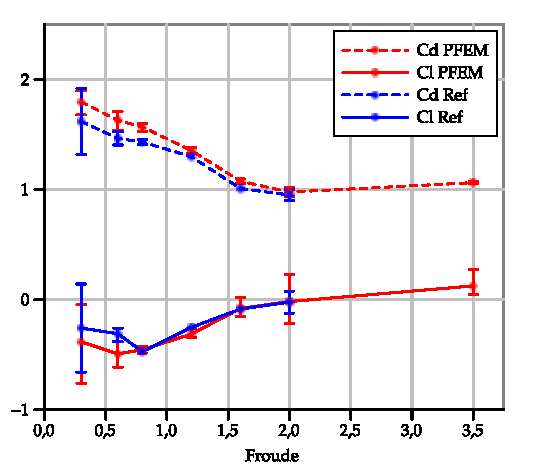
\includegraphics[width=0.95\columnwidth]{../images/CdCl_Re180_hd_0_55.pdf}
  \caption{Drag and Lift coefficients calculated with PFEM-2 compared with the reference work of Bouscasse \cite{Bouscasse14}. $Re=180$.} %, $t^*=tU/d$. }
  \label{fg:CdCl}
\end{figure}

\subsection{DMD-Analysis Results}

\begin{figure}[ht]
  \centering
  %%----primera subfigura----
  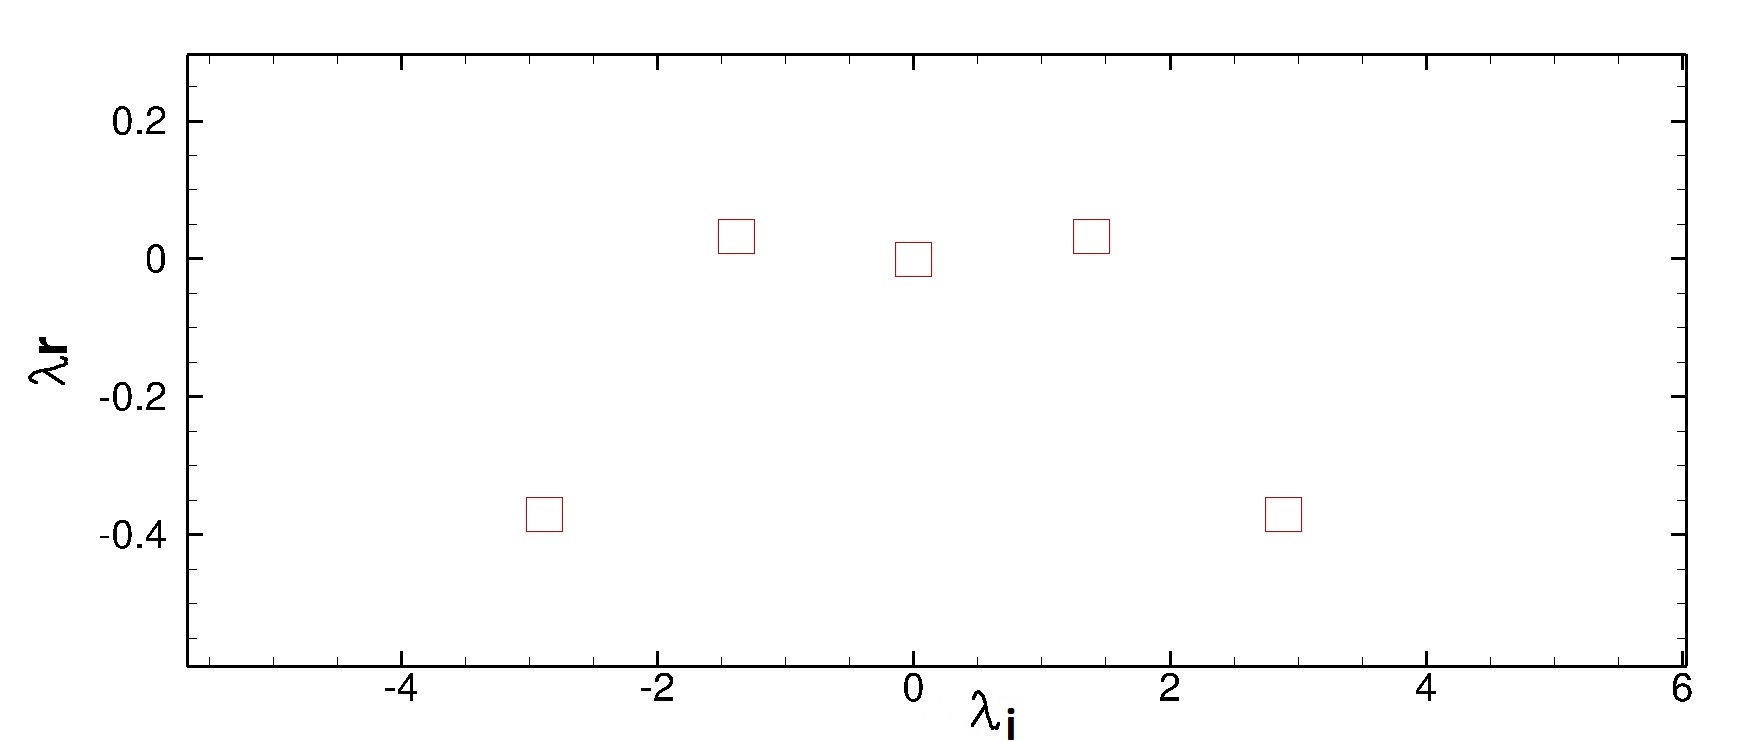
\includegraphics[width=0.95\columnwidth]{../images/modos2.jpeg}
  \caption{Spectrum obtained after the DMD analysis when 7 snapshots spaced $\Delta t=0.48$ in the time interval $[11.99,15.51]$ equivalent to $\sim0.7T$ were used at $Fr=3.5$ and $Re=180$.}
  \label{fg:DMD_spectrum}
\end{figure}

\begin{figure}[ht]
  \centering
  %%----primera subfigura----
  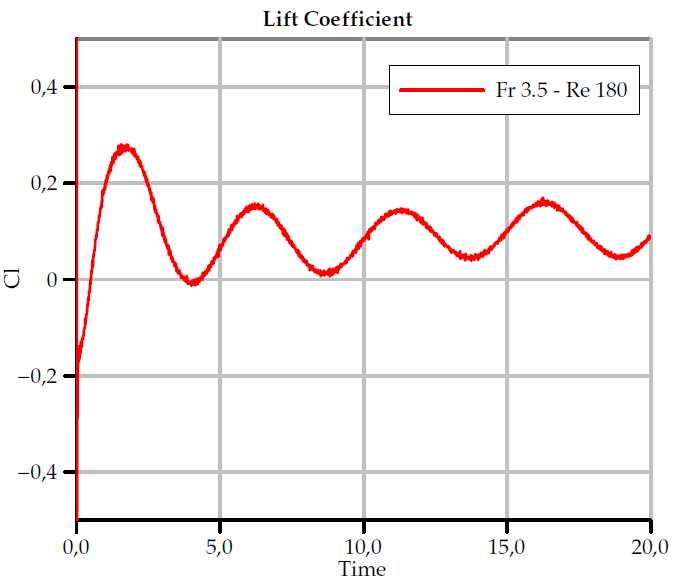
\includegraphics[width=0.95\columnwidth]{../images/ClvstimeFr035.png}
  \caption{Evolution in time of the lift coefficient $C_l$ at $Fr=3.5$ and $Re=180$ when 20s are simulated.}
  \label{fg:Liftversustime}
\end{figure}

Different DMD analyses were done for the case $Re=180$ and $Fr=3.5$, in the first case 7 snapshots spaced $\Delta t=0.48$ in the time interval $[11.99,15.51]$ equivalent to $\sim0.7T$ were used, being $T\sim5s$ the dominant period of the flow. The most relevant part of the spectrum is shown in figure \ref{fg:DMD_spectrum}, where due to the fact that the the reduced matrix $\mathbf{\widetilde{S}}$ is real, all the eigenvalues are complex conjugate. It can be observed that a pair of eigenvalues have real positive part which means that a growing instability is present in the fluid. This growing stability is not conclusive and only comes from the fact that the set of snapshots do not complete a full period, capturing the slight increasing slope when the interval $[11.99,15.51]$ is observed in figure \ref{fg:Liftversustime}, which implies a positive real part. However the imaginary part associated with the most unstable eigenvalue is $1.27$ which corresponds to a period $2\pi/\lambda_i=4.94$, which fits very well 
with the one presented in the lift coefficient evolution $T\sim5s$, see figure \ref{fg:Liftversustime}. The perturbation components associated with this dominant eigenvalue $(\lambda_r,\lambda_i)=(0.05,1.5)$ are plot in figure \ref{fg:mode}, where the typical shape associated to a vortex shedding mode can be observed. To the authors knowledge this is the first time where a typical vortex shedding mode is observed in the presence of free surface. It can be observed how the mode is deformed due to the free surface shape when compared to the typical vortex shedding mode when no free surface has been introduced, see figure \ref{fg:mode Nofreesurface} from a typical biglobal computation at $Re=60$. A second DMD analysis was performed using 40 snapshots spaced $\Delta t=0.16$ in the time interval $[11.9,18.3]$ equivalent to $\sim 1.3T$, in this case the most dominant mode shifted its real part to the stable part of the spectrum, while the frequency is fixed to similar to the ones obtained in the first case. The 
decrease of the real part of the dominant mode can be explained due to the fact that the snapshots have been taken during a longer interval where the growing tendency is not so clearly observed. However the structure of the mode barely changes as can be appreciated when figures \ref{fg:DMDglobal2} and \ref{fg:DMDglobal3} are compared. Finally, a third analysis 20 snapshots spaced $\Delta t=0.5$ in the time interval $[19.98,30.48]$ equivalent to $\sim2T$ were used. If the total simulation time is extended from 20s to 50s, the growing tendency of the lift coefficient is clearly observed, see figure \ref{fg:Liftlonger}. The result from the DMD analysis captures this growing tendency and shifts the dominant mode back to the unstable part of the plane $\lambda_r<0$, see figure \ref{fg:DMDglobal} keeping the frequency of the mode at similar values as the previous analyses. As before, the structure of the dominant mode reamins unchanged, see figure \ref{fg:DMDglobal4}. The complexity of the flow can be appreciated 
when a secondary mode is plot, see figure \ref{fg:DMDglobal5}, where the higher temporal frequency implies a more complex structure in the mode.



\begin{figure}[ht]
  \centering
  %%----primera subfigura----
  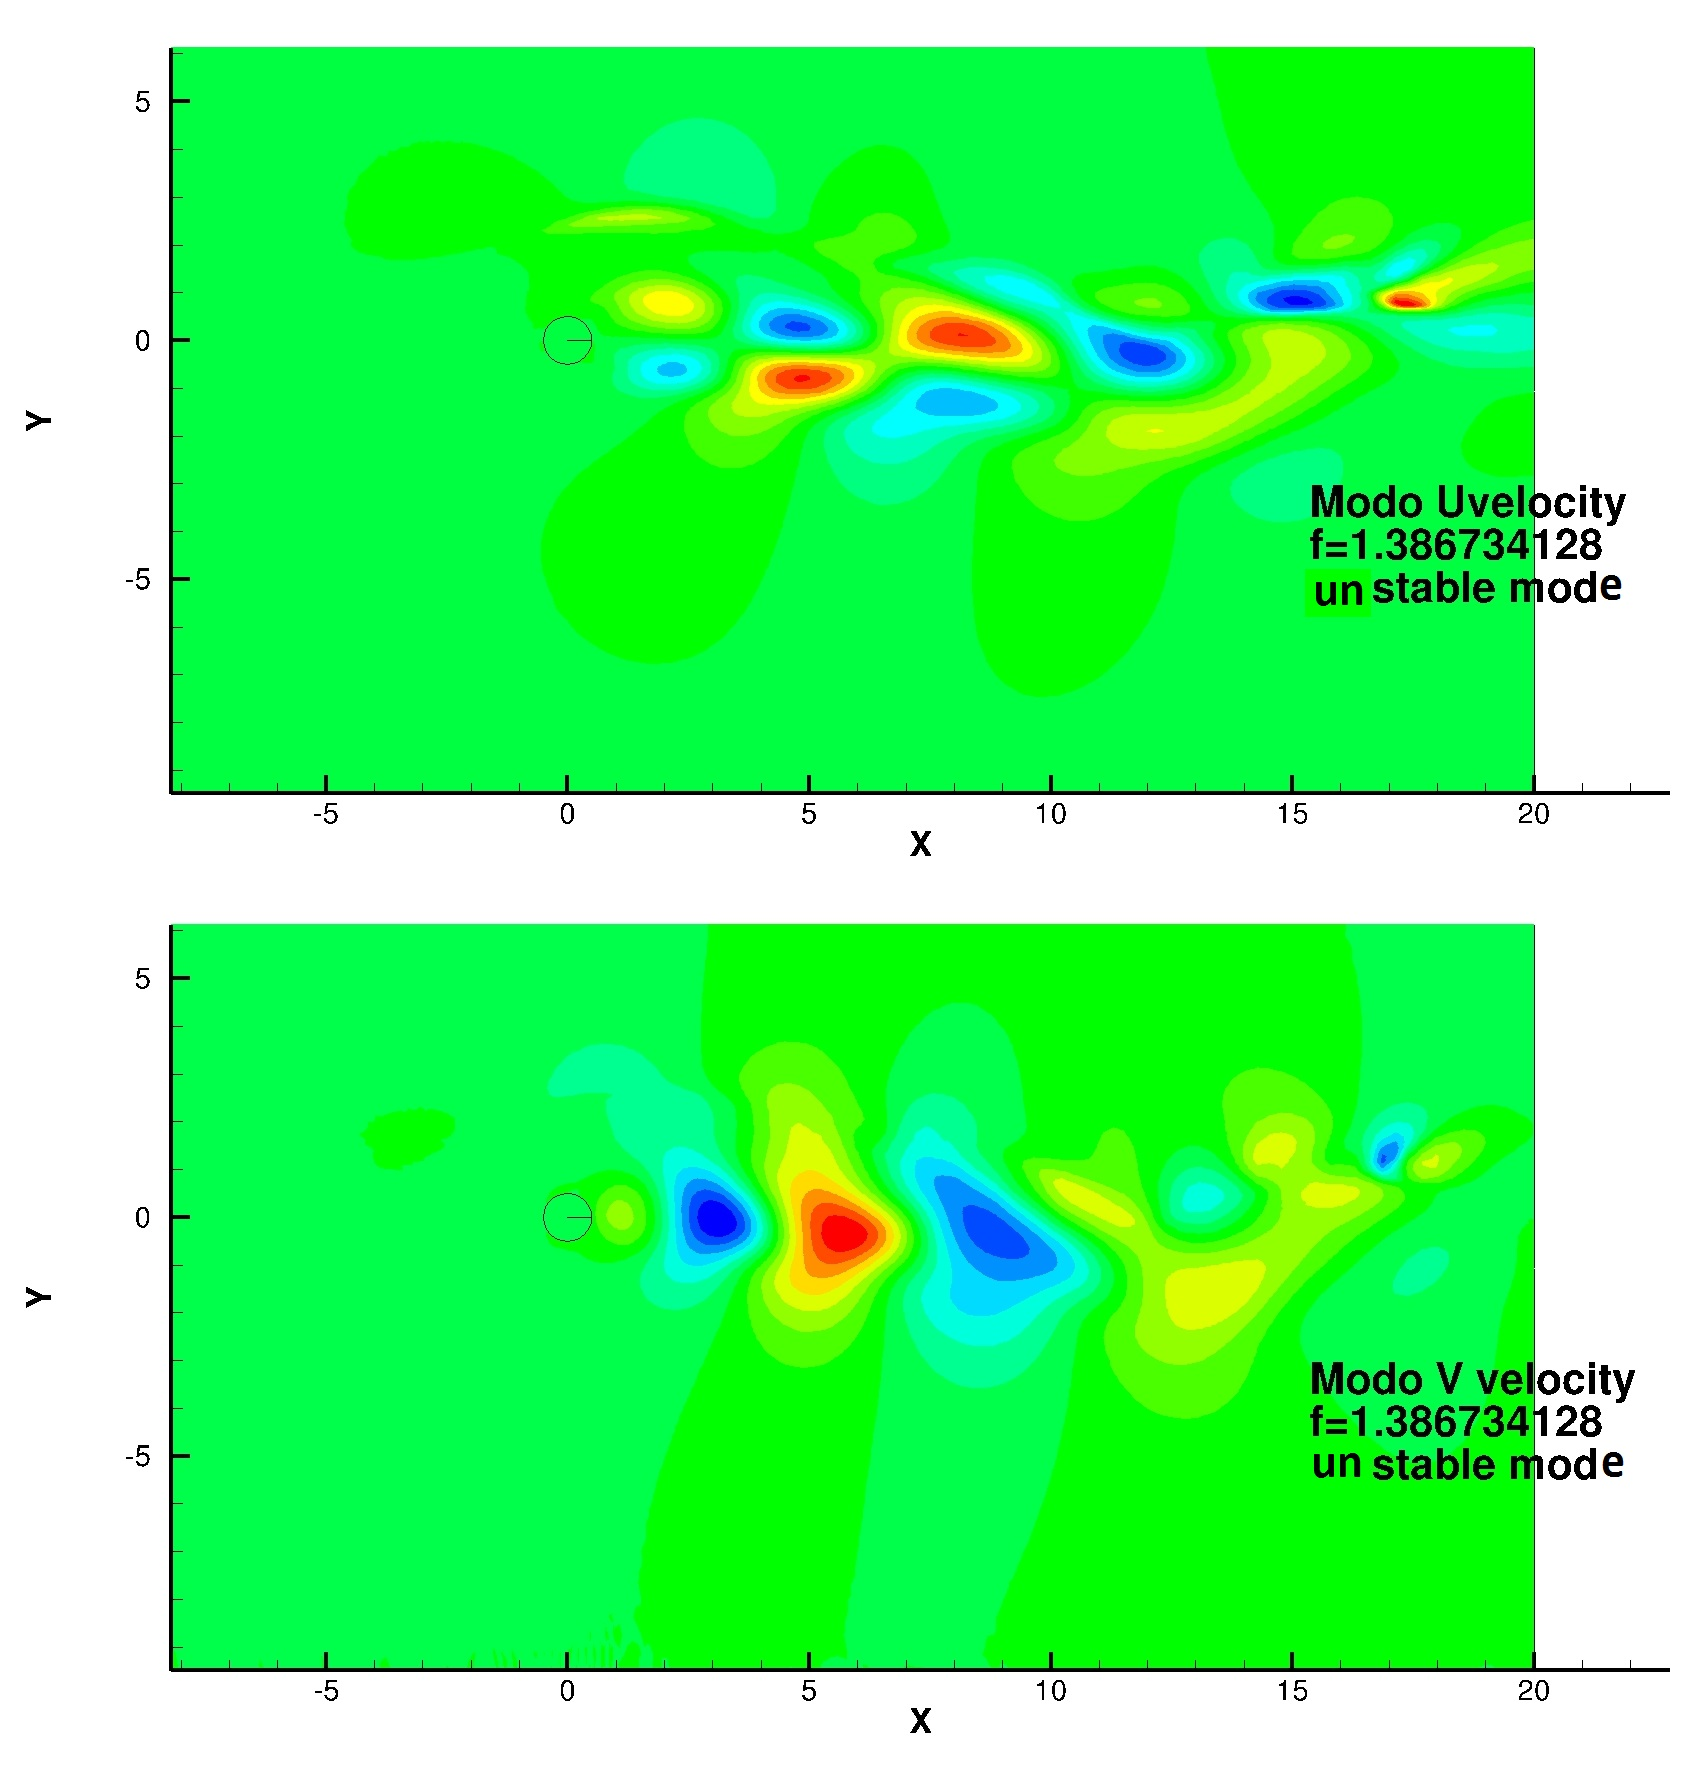
\includegraphics[width=1\columnwidth]{../images/modos3.jpeg}
  \caption{Perturbation velocity components of the most unstable mode obtained after the first DMD analysis when 7 snapshots spaced $\Delta t=0.48$ in the time interval $[11.99,15.51]$ equivalent to $\sim0.7T$ at $Fr=3.5$ and $Re=180$. Top: horizontal velocity, bottom: vertical velocity component.}
  \label{fg:mode}
\end{figure}

\begin{figure}[ht]
  \centering
  %%----primera subfigura----
  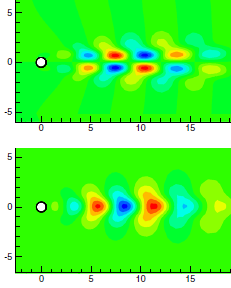
\includegraphics[width=0.95\columnwidth]{../images/Typical_cilinder_mode.png}
  \caption{Perturbation velocity components of the most unstable mode obtained by biglobal analysis when the $Re=60$ and no free surface has been considered. Top: horizontal velocity, bottom: vertical velocity component.}
  \label{fg:mode Nofreesurface}
\end{figure}

\begin{figure}[ht]
  \centering
  %%----primera subfigura----
  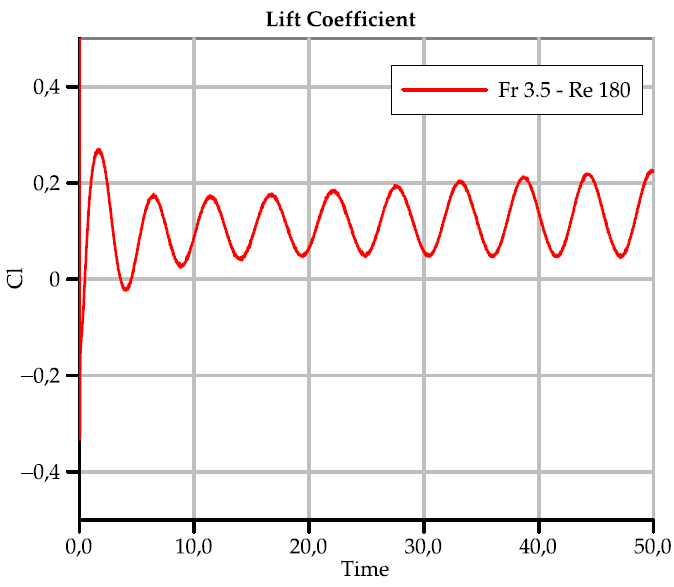
\includegraphics[width=0.95\columnwidth]{../images/LongerCl.png}
  \caption{Evolution in time of the lift coefficient $C_l$ at $Fr=3.5$ $Re=180$ when 50s are simulated.}
  \label{fg:Liftlonger}
\end{figure}

\begin{figure}[ht]
  \centering
  %%----primera subfigura----
  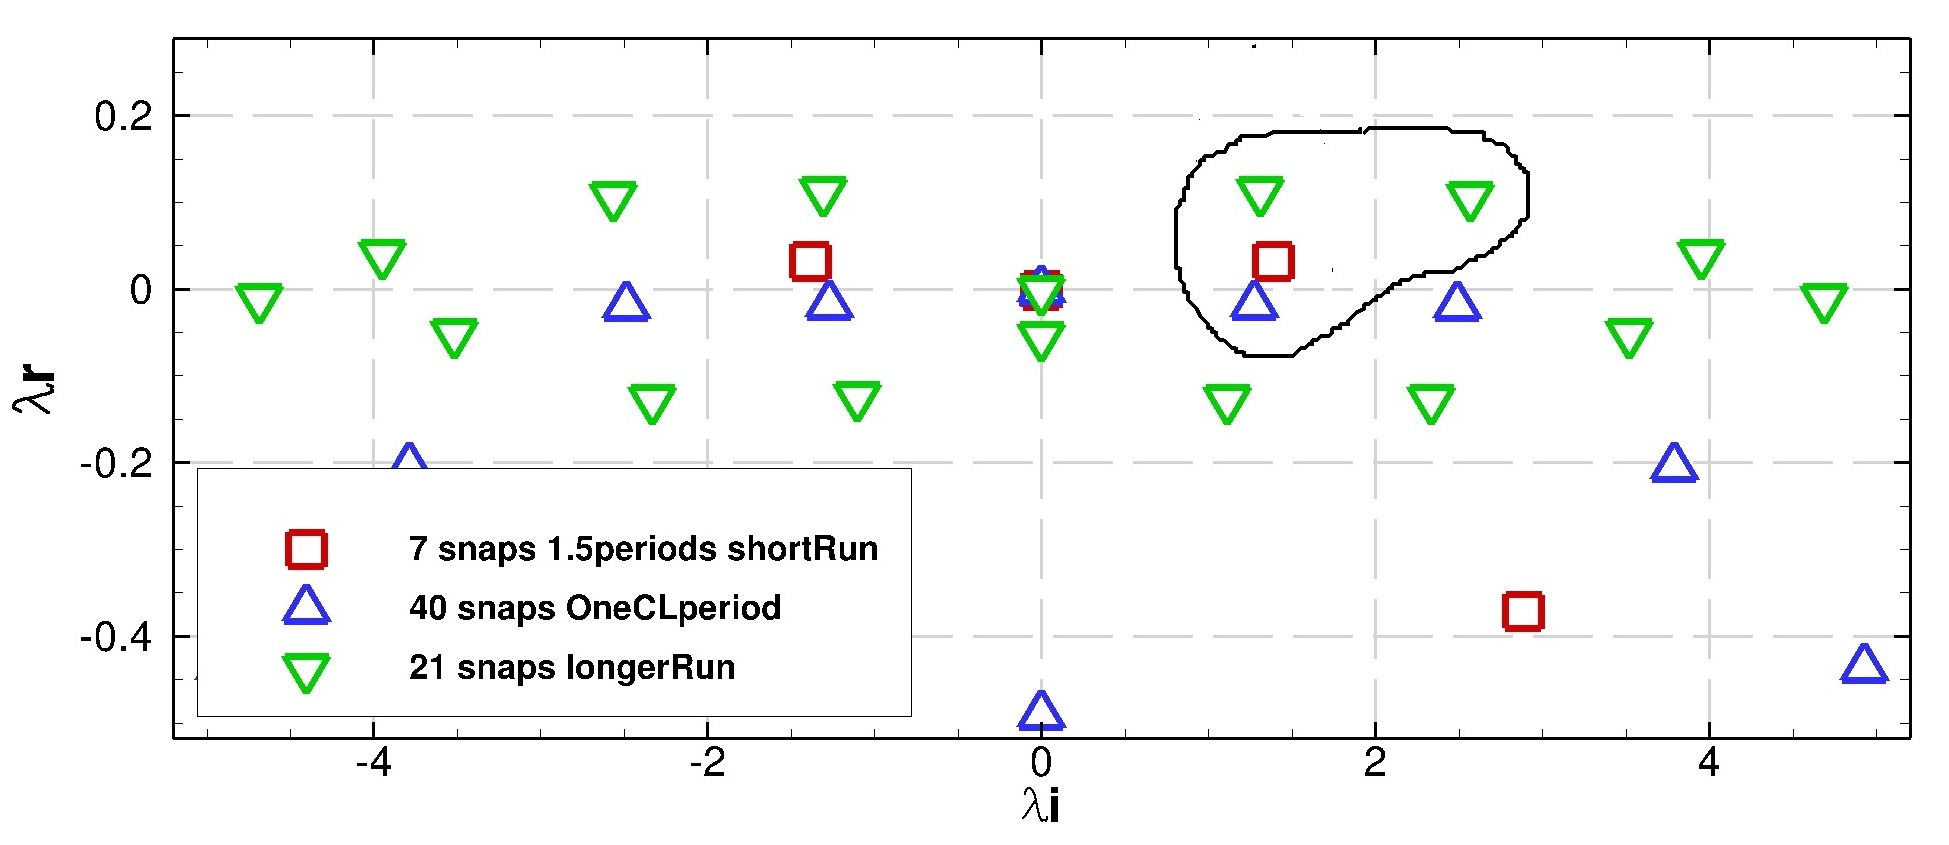
\includegraphics[width=0.95\columnwidth]{../images/7vs40vslongersnaps.jpg}
  \caption{Comparative spectra obtained after the three DMD analysis at $Fr=3.5$ and $Re=180$}
  \label{fg:DMDglobal}
\end{figure}

\begin{figure}[ht]
  \centering
  %%----primera subfigura----
  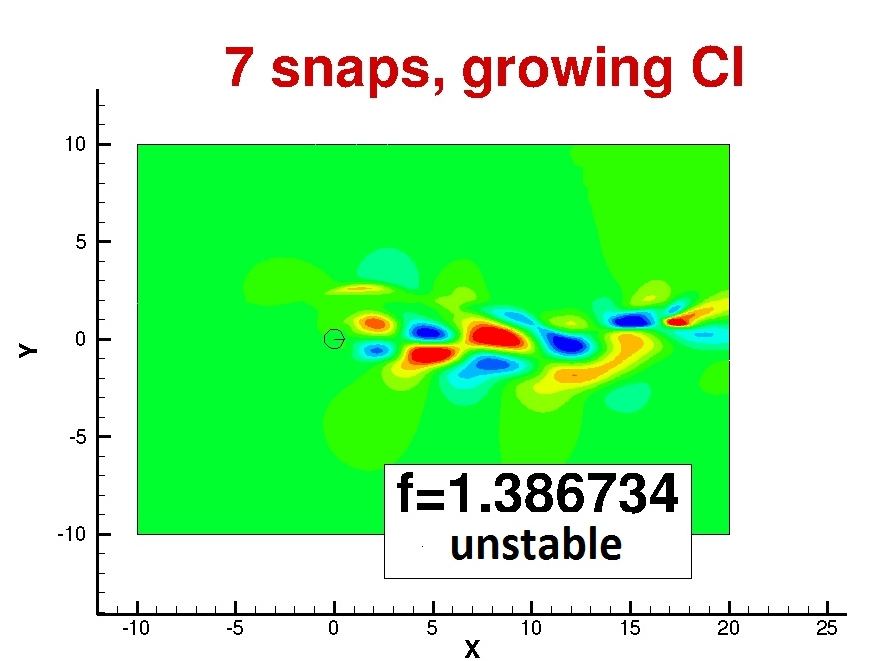
\includegraphics[width=0.95\columnwidth]{../images/modo1u.png}
  \caption{Horizontal velocity component of the unstable mode represented by a red square inside the rounded area in figure \ref{fg:DMDglobal}.}
  \label{fg:DMDglobal2}
\end{figure}
\begin{figure}[ht]
  \centering
  %%----primera subfigura----
  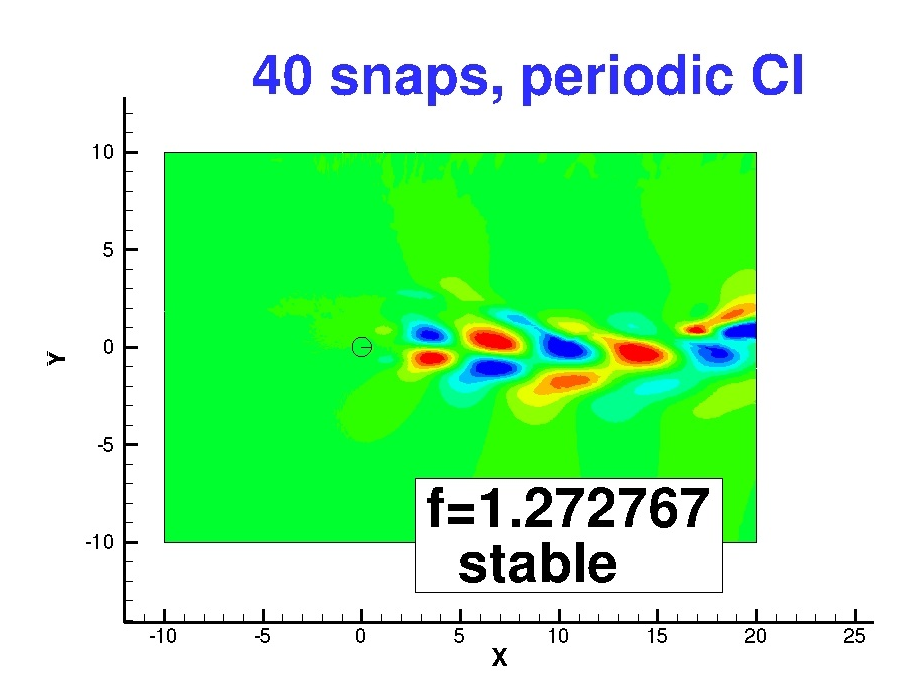
\includegraphics[width=0.95\columnwidth]{../images/modo2u.png}
  \caption{Horizontal velocity component of the stable mode represented by a blue triangle inside the rounded area in figure \ref{fg:DMDglobal}.}
  \label{fg:DMDglobal3}
\end{figure}

\begin{figure}[ht]
  \centering
  %%----primera subfigura----
  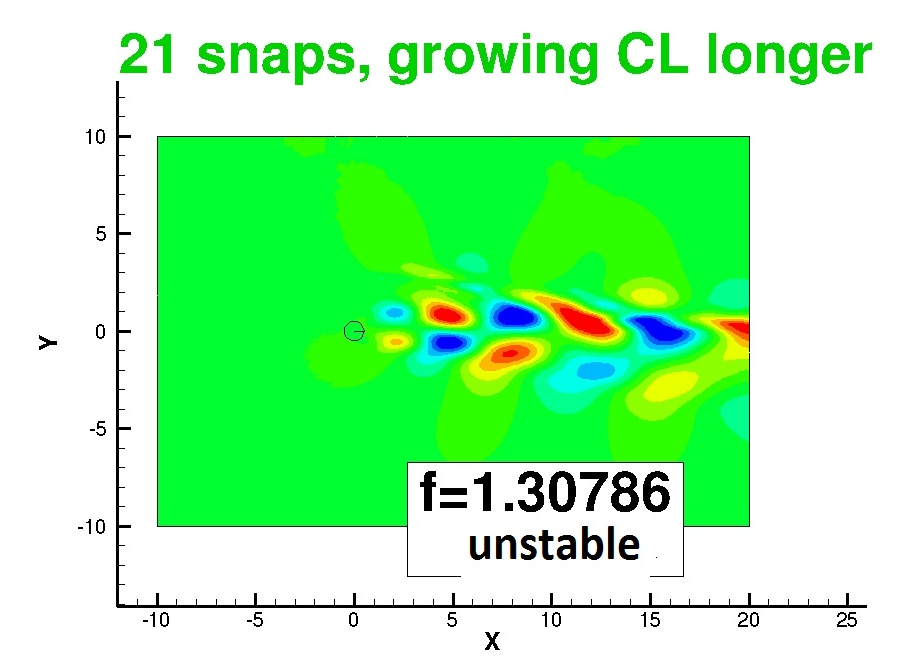
\includegraphics[width=0.95\columnwidth]{../images/modo3u.png}
  \caption{Horizontal velocity component of the most unstable mode represented by a green triangle inside the rounded area in figure \ref{fg:DMDglobal}.}
  \label{fg:DMDglobal4}
\end{figure}
\begin{figure}[ht]
  \centering
  %%----primera subfigura----
  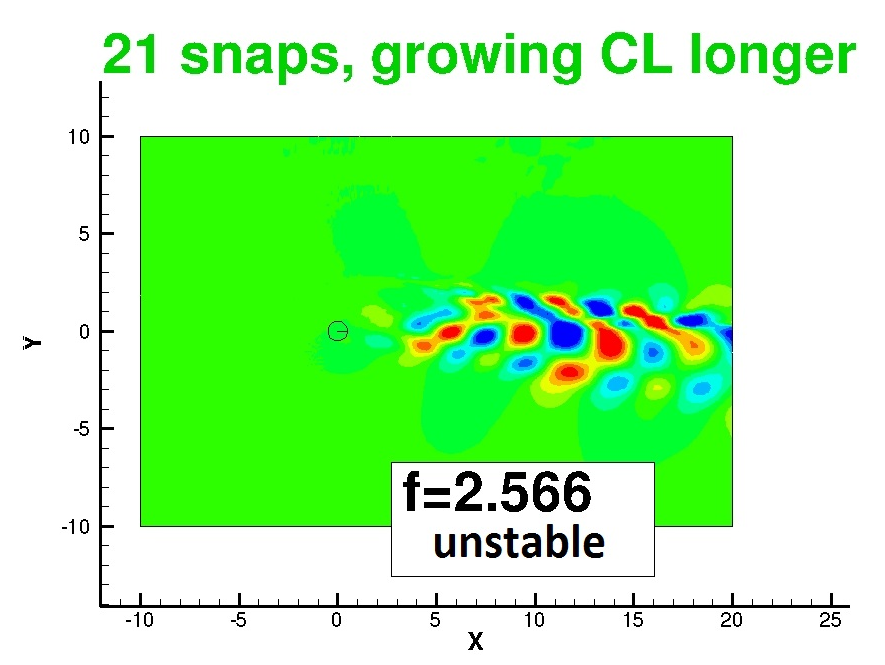
\includegraphics[width=0.95\columnwidth]{../images/modo4u.png}
  \caption{Horizontal velocity component of the secondary unstable mode represented by a green triangle inside the rounded area in figure \ref{fg:DMDglobal}.}
  \label{fg:DMDglobal5}
\end{figure} 